The example is illustrated below, in which we can see that no matter which minimum spanning trees we choose, the $m_3$ of each minimum spanning trees is indentical. The edges colored red are the minimum spanning tree.
\begin{figure}[H]
	\centering
	\subfigure[A possible minimum spanning tree]{
	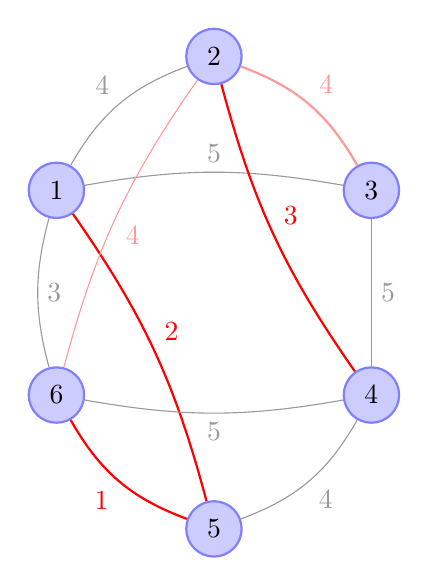
\begin{tikzpicture}
		[place1/.style={circle,draw=blue!50,fill=blue!20,thick,
inner sep=0pt,minimum size=20pt},
		place2/.style={circle,draw=green!60,fill=green!30,thick,
inner sep=0pt,minimum size=40pt},
		textstyle/.style={},
		bend angle=45,
		edgestyle/.style={-,shorten <=1pt,>=stealth’,semithick}]
		\node at (-2.0, 1.3) (1) [place1] {$1$};
		\node at (0.0, 3.0) (2) [place1] {$2$}
			edge [-,bend right=20,black!40] node[auto,swap] {$4$} (1);
		\node at (2.0, 1.3) (3) [place1] {$3$}
			edge [-,bend right=10,black!40] node[auto,swap] {$5$} (1)
			edge [-,bend right=20,red!40,thick] node[auto,swap] {$4$} (2);
		\node at (2.0, -1.3) (4) [place1] {$4$}
			edge [-,bend left=10,red,thick] node[auto,swap] {$3$} (2)
			edge [-,bend right=0,black!40] node[auto,swap] {$5$} (3);
		\node at (0.0, -3.0) (5) [place1] {$5$}
			edge [-,bend right=20,black!40] node[auto,swap] {$4$} (4)
			edge [-,bend right=10,red,thick] node[auto,swap] {$2$} (1);
		\node at (-2.0, -1.3) (6) [place1] {$6$}
			edge [-,bend right=20,red,thick] node[auto,swap] {$1$} (5)
			edge [-,bend right=10,black!40] node[auto,swap] {$5$} (4)
			edge [-,bend left=10,red!40] node[auto,swap] {$4$} (2)
			edge [-,black!40,bend left=15] node[auto,swap] {$3$} (1);
	\end{tikzpicture}
	}
	\subfigure[Another possible version of the minimum spanning tree]{
	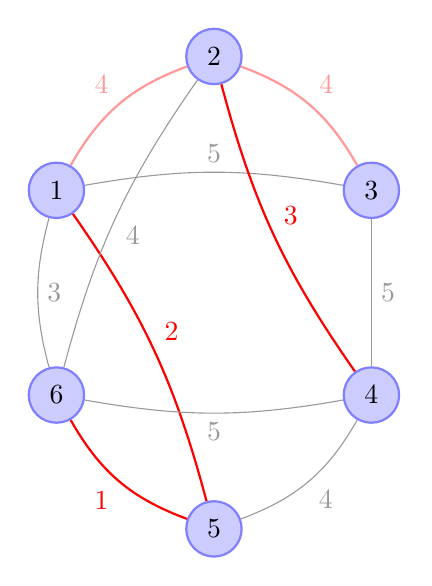
\begin{tikzpicture}
		[place1/.style={circle,draw=blue!50,fill=blue!20,thick,
inner sep=0pt,minimum size=20pt},
		place2/.style={circle,draw=green!60,fill=green!30,thick,
inner sep=0pt,minimum size=40pt},
		textstyle/.style={},
		bend angle=45,
		edgestyle/.style={-,shorten <=1pt,>=stealth’,semithick}]
		\node at (-2.0, 1.3) (1) [place1] {$1$};
		\node at (0.0, 3.0) (2) [place1] {$2$}
			edge [-,bend right=20,red!40,thick] node[auto,swap] {$4$} (1);
		\node at (2.0, 1.3) (3) [place1] {$3$}
			edge [-,bend right=10,black!40] node[auto,swap] {$5$} (1)
			edge [-,bend right=20,red!40,thick] node[auto,swap] {$4$} (2);
		\node at (2.0, -1.3) (4) [place1] {$4$}
			edge [-,bend left=10,red,thick] node[auto,swap] {$3$} (2)
			edge [-,bend right=0,black!40] node[auto,swap] {$5$} (3);
		\node at (0.0, -3.0) (5) [place1] {$5$}
			edge [-,bend right=20,black!40] node[auto,swap] {$4$} (4)
			edge [-,bend right=10,red,thick] node[auto,swap] {$2$} (1);
		\node at (-2.0, -1.3) (6) [place1] {$6$}
			edge [-,bend right=20,red,thick] node[auto,swap] {$1$} (5)
			edge [-,bend right=10,black!40] node[auto,swap] {$5$} (4)
			edge [-,bend left=10,black!40] node[auto,swap] {$4$} (2)
			edge [-,black!40,bend left=15] node[auto,swap] {$3$} (1);;
	\end{tikzpicture}
	}
	\subfigure[The remained possible minimum spanning tree]{
	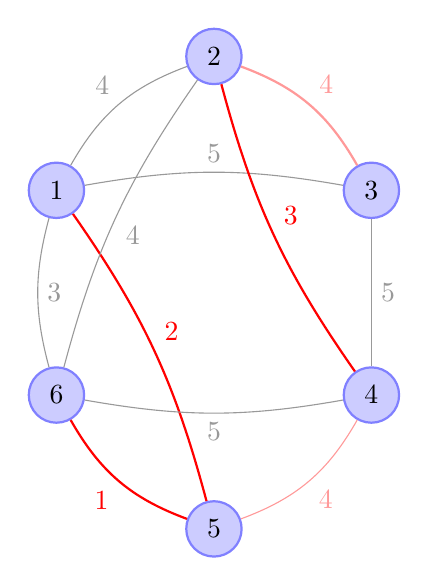
\begin{tikzpicture}
		[place1/.style={circle,draw=blue!50,fill=blue!20,thick,
inner sep=0pt,minimum size=20pt},
		place2/.style={circle,draw=green!60,fill=green!30,thick,
inner sep=0pt,minimum size=40pt},
		textstyle/.style={},
		bend angle=45,
		edgestyle/.style={-,shorten <=1pt,>=stealth’,semithick}]
		\node at (-2.0, 1.3) (1) [place1] {$1$};
		\node at (0.0, 3.0) (2) [place1] {$2$}
			edge [-,bend right=20,black!40] node[auto,swap] {$4$} (1);
		\node at (2.0, 1.3) (3) [place1] {$3$}
			edge [-,bend right=10,black!40] node[auto,swap] {$5$} (1)
			edge [-,bend right=20,red!40,thick] node[auto,swap] {$4$} (2);
		\node at (2.0, -1.3) (4) [place1] {$4$}
			edge [-,bend left=10,red,thick] node[auto,swap] {$3$} (2)
			edge [-,bend right=0,black!40] node[auto,swap] {$5$} (3);
		\node at (0.0, -3.0) (5) [place1] {$5$}
			edge [-,bend right=20,red!40] node[auto,swap] {$4$} (4)
			edge [-,bend right=10,red,thick] node[auto,swap] {$2$} (1);
		\node at (-2.0, -1.3) (6) [place1] {$6$}
			edge [-,bend right=20,red,thick] node[auto,swap] {$1$} (5)
			edge [-,bend right=10,black!40] node[auto,swap] {$5$} (4)
			edge [-,bend left=10,black!40] node[auto,swap] {$4$} (2)
			edge [-,black!40,bend left=15] node[auto,swap] {$3$} (1);
	\end{tikzpicture}
	}
	\caption{Three possible minimum spanning trees and its $m_3$}
\end{figure}

